\documentclass[17pt,a4paper,landscape]{extarticle}
\usepackage[margin=1.45cm,top=0.5cm,bottom=1.0cm]{geometry}
\usepackage{amsmath}
\usepackage{amssymb}
\usepackage{tasks}
\usepackage{tikz}
\usepackage{xcolor}
\usepackage[sfdefault,lf]{FiraSans}
\renewcommand{\familydefault}{\sfdefault}
\setlength{\parindent}{0pt}
\pagestyle{empty}
\renewcommand{\arraystretch}{1.15}
\everymath{\displaystyle}
\begin{document}
\sffamily
\boldmath
{\LARGE \textbf{Drawing parabola from given equation — Foundation}}\\[0.2em]
{\large Use the numbered blank grids. For each one, make a table of values, plot the points, then draw the parabola.}
\begin{center}
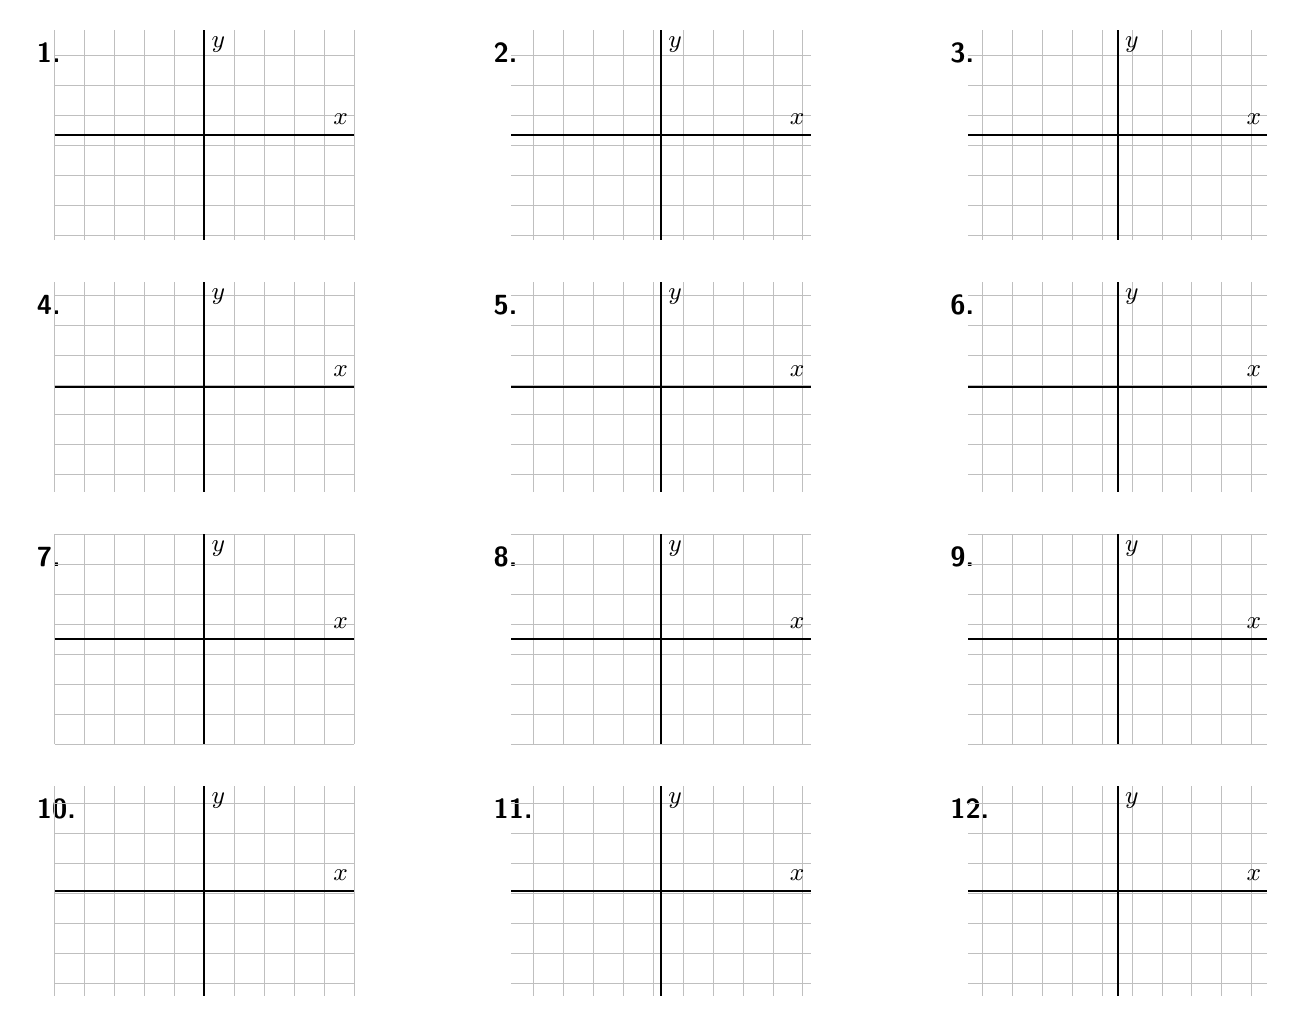
\begin{tikzpicture}[x=1cm,y=1cm]
\node[anchor=west,font=\bfseries] at (-0.35,12.579999999999998) {1.};
\draw[step=0.38cm,very thin,color=gray!50] (0.0,10.2) grid (3.8,12.86);
\draw[thick] (1.9,10.2) -- (1.9,12.86);
\draw[thick] (0.0,11.53) -- (3.8,11.53);
\node[font=\small] at (3.63,11.729999999999999) {$x$};
\node[font=\small] at (2.08,12.68) {$y$};
\node[anchor=west,font=\bfseries] at (5.45,12.579999999999998) {2.};
\draw[step=0.38cm,very thin,color=gray!50] (5.8,10.2) grid (9.6,12.86);
\draw[thick] (7.699999999999999,10.2) -- (7.699999999999999,12.86);
\draw[thick] (5.8,11.53) -- (9.6,11.53);
\node[font=\small] at (9.43,11.729999999999999) {$x$};
\node[font=\small] at (7.88,12.68) {$y$};
\node[anchor=west,font=\bfseries] at (11.25,12.579999999999998) {3.};
\draw[step=0.38cm,very thin,color=gray!50] (11.6,10.2) grid (15.399999999999999,12.86);
\draw[thick] (13.5,10.2) -- (13.5,12.86);
\draw[thick] (11.6,11.53) -- (15.399999999999999,11.53);
\node[font=\small] at (15.23,11.729999999999999) {$x$};
\node[font=\small] at (13.68,12.68) {$y$};
\node[anchor=west,font=\bfseries] at (-0.35,9.379999999999999) {4.};
\draw[step=0.38cm,very thin,color=gray!50] (0.0,7.0) grid (3.8,9.66);
\draw[thick] (1.9,7.0) -- (1.9,9.66);
\draw[thick] (0.0,8.33) -- (3.8,8.33);
\node[font=\small] at (3.63,8.53) {$x$};
\node[font=\small] at (2.08,9.48) {$y$};
\node[anchor=west,font=\bfseries] at (5.45,9.379999999999999) {5.};
\draw[step=0.38cm,very thin,color=gray!50] (5.8,7.0) grid (9.6,9.66);
\draw[thick] (7.699999999999999,7.0) -- (7.699999999999999,9.66);
\draw[thick] (5.8,8.33) -- (9.6,8.33);
\node[font=\small] at (9.43,8.53) {$x$};
\node[font=\small] at (7.88,9.48) {$y$};
\node[anchor=west,font=\bfseries] at (11.25,9.379999999999999) {6.};
\draw[step=0.38cm,very thin,color=gray!50] (11.6,7.0) grid (15.399999999999999,9.66);
\draw[thick] (13.5,7.0) -- (13.5,9.66);
\draw[thick] (11.6,8.33) -- (15.399999999999999,8.33);
\node[font=\small] at (15.23,8.53) {$x$};
\node[font=\small] at (13.68,9.48) {$y$};
\node[anchor=west,font=\bfseries] at (-0.35,6.18) {7.};
\draw[step=0.38cm,very thin,color=gray!50] (0.0,3.8) grid (3.8,6.46);
\draw[thick] (1.9,3.8) -- (1.9,6.46);
\draw[thick] (0.0,5.13) -- (3.8,5.13);
\node[font=\small] at (3.63,5.33) {$x$};
\node[font=\small] at (2.08,6.279999999999999) {$y$};
\node[anchor=west,font=\bfseries] at (5.45,6.18) {8.};
\draw[step=0.38cm,very thin,color=gray!50] (5.8,3.8) grid (9.6,6.46);
\draw[thick] (7.699999999999999,3.8) -- (7.699999999999999,6.46);
\draw[thick] (5.8,5.13) -- (9.6,5.13);
\node[font=\small] at (9.43,5.33) {$x$};
\node[font=\small] at (7.88,6.279999999999999) {$y$};
\node[anchor=west,font=\bfseries] at (11.25,6.18) {9.};
\draw[step=0.38cm,very thin,color=gray!50] (11.6,3.8) grid (15.399999999999999,6.46);
\draw[thick] (13.5,3.8) -- (13.5,6.46);
\draw[thick] (11.6,5.13) -- (15.399999999999999,5.13);
\node[font=\small] at (15.23,5.33) {$x$};
\node[font=\small] at (13.68,6.279999999999999) {$y$};
\node[anchor=west,font=\bfseries] at (-0.35,2.98) {10.};
\draw[step=0.38cm,very thin,color=gray!50] (0.0,0.6) grid (3.8,3.2600000000000002);
\draw[thick] (1.9,0.6) -- (1.9,3.2600000000000002);
\draw[thick] (0.0,1.9300000000000002) -- (3.8,1.9300000000000002);
\node[font=\small] at (3.63,2.13) {$x$};
\node[font=\small] at (2.08,3.08) {$y$};
\node[anchor=west,font=\bfseries] at (5.45,2.98) {11.};
\draw[step=0.38cm,very thin,color=gray!50] (5.8,0.6) grid (9.6,3.2600000000000002);
\draw[thick] (7.699999999999999,0.6) -- (7.699999999999999,3.2600000000000002);
\draw[thick] (5.8,1.9300000000000002) -- (9.6,1.9300000000000002);
\node[font=\small] at (9.43,2.13) {$x$};
\node[font=\small] at (7.88,3.08) {$y$};
\node[anchor=west,font=\bfseries] at (11.25,2.98) {12.};
\draw[step=0.38cm,very thin,color=gray!50] (11.6,0.6) grid (15.399999999999999,3.2600000000000002);
\draw[thick] (13.5,0.6) -- (13.5,3.2600000000000002);
\draw[thick] (11.6,1.9300000000000002) -- (15.399999999999999,1.9300000000000002);
\node[font=\small] at (15.23,2.13) {$x$};
\node[font=\small] at (13.68,3.08) {$y$};
\end{tikzpicture}
\end{center}
\settasks{label=\textbf{\arabic*.}, label-width=2.2em, item-indent=2.95em, column-sep=1.3cm, after-item-skip=0.9em}
\begin{tasks}(3)
\task Draw \mbox{$ y=x^2 $}.
\task Draw \mbox{$ y=x^2+1 $}.
\task Draw \mbox{$ y=x^2-2 $}.
\task Draw \mbox{$ y=(x-1)^2 $}.
\task Draw \mbox{$ y=(x+2)^2 $}.
\task Draw \mbox{$ y=-x^2 $}.
\task Draw \mbox{$ y=-x^2+3 $}.
\task Draw \mbox{$ y=2x^2 $}.
\task Draw \mbox{$ y=\frac{1}{2}x^2 $}.
\task Draw \mbox{$ y=x^2+2x $}.
\task Draw \mbox{$ y=x^2-4x $}.
\task Draw \mbox{$ y=x^2+4x+3 $}.
\end{tasks}
\end{document}
